\section{Exceptions \& Interrupts}
% ========================================
% 
% ========================================
\begin{frame}{Exceptions \& Interrupts}{}
\begin{itemize}
\item Exceptions and interrupts are unexpected events that disrupt the normal execution of a program. 
\item They are not \code{branch} or \code{jump} instructions executed in a program. 
\item They transfer the control of the \ac{CPU} to a special program, known as \alertblue{handler}.
\item Exceptions and interruptions are mistakenly used as interchangeable terms. However, they differ from each other.
\item The difference between an exception and an interrupt is the source that triggered the change in the flow control. 
\end{itemize}
\end{frame} 

% ========================================
% 
% ========================================
\begin{frame}{Exceptions \& Interrupts}{}
\begin{figure}
\centering
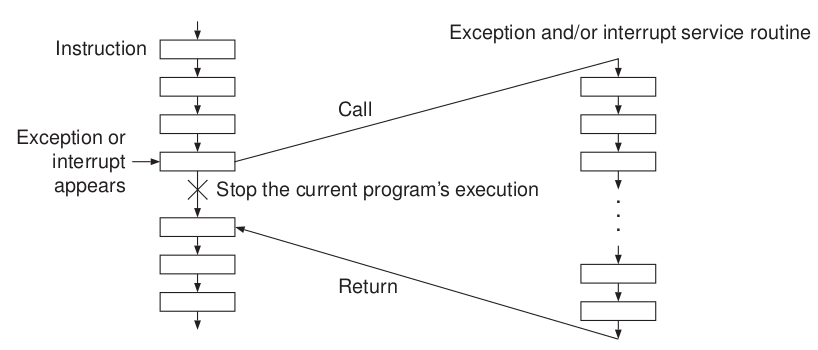
\includegraphics[width=\textwidth]{interrupt_basic}
\caption{Exceptions and interruptions flow control.}
\label{Figure:Interruption_basic}
\end{figure}
\end{frame}

% ========================================
% 
% ========================================
\begin{frame}{Exceptions \& Interrupts}{}
\begin{itemize}
\item \alertblue{Exceptions} are \alertblue{synchronous} unscheduled events that occur \alertblue{internally} to the processor.
\pauseprint
  \begin{itemize}
  \item Arithmetic overflow.
  \item Unsupported instruction.
  \end{itemize}
\pauseprint
\item \alertred{Interrupts} are \alertred{asynchronous} unscheduled events that occur \alertred{externally} to the processor.
\pauseprint
  \begin{itemize}
  \item \ac{IO} devices such as keyboard or mouse.
  \item Timers.
  \end{itemize}
\end{itemize}
\end{frame} 

% ========================================
% 
% ========================================
\begin{frame}{Exceptions \& Interrupts}{}
Is the following example an interrupt or an exception?
\begin{itemize}
\item Your current \ac{MIPS} design.
  \begin{itemize}
  \item R-Type and I-Type instructions are supported.
  \pauseprint
  \item What about J-Type instructions?
  \item What would happen in your design if the \ac{uP} receives a \code{jump} instruction?
  \end{itemize}
\end{itemize}
\end{frame} 

% ========================================
% 
% ========================================
\begin{frame}{Exceptions \& Interrupts}{}
\begin{itemize}
\item \acp{uP} usually rely on a special register for handling exceptions.
\item This register is the \ac{EPC}.
\item \ac{EPC} stores the address of the instruction that caused the exception before transferring flow control to the program handler.
\item The handler may then provide service to the offending program with a predefined action.
\item If the handler does not terminate the main program execution, it uses the \ac{EPC} in order to return control to the main program and resume its execution.
\end{itemize}
\end{frame}

% ========================================
% 
% ========================================
\begin{frame}{Exceptions \& Interrupts}{}
\begin{itemize}
\item There are two ways to transfer control to the handlers.
  \begin{itemize}
  \item Polled.
  \item Vectored.
  \end{itemize}
\end{itemize}
\end{frame}

% ========================================
% 
% ========================================
\begin{frame}{Exceptions \& Interrupts}{}
\alertblue{Polled exceptions/interrupts}
\begin{itemize}
\item \ac{MIPS} \ac{uA} provides a status register, called \textbf{Cause Register}, which holds a field that indicates the reason for the exception/interrupt.
\end{itemize}
\begin{figure}
\centering
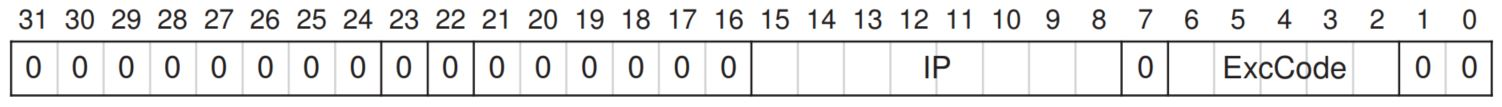
\includegraphics[width=\textwidth]{cause_register}
\caption{Cause register example.}
\label{Figure:CauseRegister}
\end{figure}
\end{frame}

% ========================================
% 
% ========================================
\begin{frame}{Exceptions \& Interrupts}{}
\begin{figure}
\centering
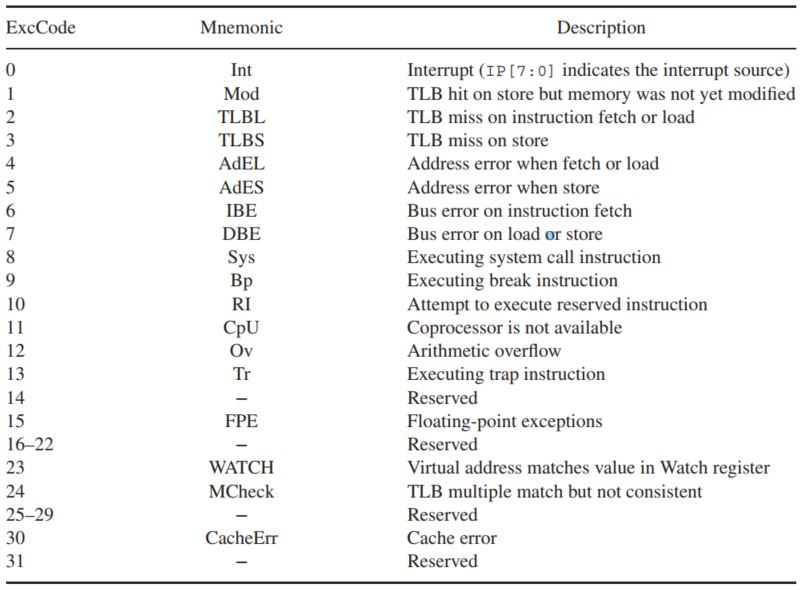
\includegraphics[scale=0.59]{ExcCode}
\vspace{-10pt}
\caption{Causes of exceptions in \ac{MIPS} \ac{uA}.}
\label{Figure:ExcCode}
\end{figure}
\end{frame}

% ========================================
% 
% ========================================
\begin{frame}{Exceptions \& Interrupts}{}
\begin{itemize}
\item In polled exceptions/interrupts, the control transfer is done in two steps.
\begin{enumerate}
\item Control is transferred to a common entry address.
\item Control is then transferred to an individual address corresponding to the ExcCode handler.
\end{enumerate}
\item In contrast, in \alertblue{vectored exceptions/interrupts}, the address to which control is transferred is determined by the cause of the exception.
\item This is done by hardware by generating a unique vector and an attached address corresponding to the address of the handler.
\end{itemize}
\end{frame}


% ========================================
% 
% ========================================
\begin{frame}{Exceptions \& Interrupts}{}
\begin{figure}
\centering
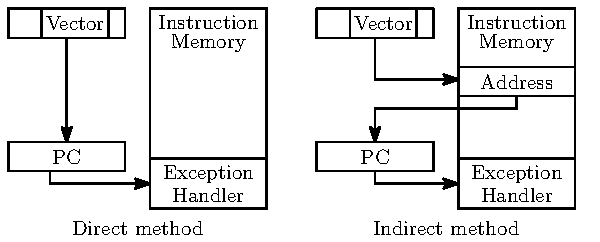
\includegraphics[width=\textwidth]{vectored_interrupt}
\caption{Mechanisms for vectored interrupts.}
\label{Figure:vectored_interrupt}
\end{figure}
\end{frame}


% ========================================
% 
% ========================================
\begin{frame}{Exceptions \& Interrupts}{}
\begin{itemize}
\item How does a handler return the control to the main program?
\pauseprint
\item The return address must be saved prior entering the handler's routine.
\item Based on the \acp{ISA}, the return address may be saved to
\begin{itemize}
\item A general-purpose register.
\item A special register.
\item Stack memory.
\end{itemize} 

\end{itemize}
\end{frame}


% ========================================
% 
% ========================================
\begin{frame}{Exceptions \& Interrupts}{}
\begin{itemize}
\item Exceptions store the current \ac{PC} value.
\begin{itemize}
\item This is done in case the offending instructions needs to be executed again.
\end{itemize}
\item Interrupts, on the other hand, store the \alertblue{next} \ac{PC} value.
\begin{itemize}
\item Current instruction is completed before transferring control to handler.
\end{itemize}
\end{itemize}
\end{frame}

% ========================================
% 
% ========================================
\begin{frame}{Exceptions \& Interrupts}{}
\begin{figure}
\centering
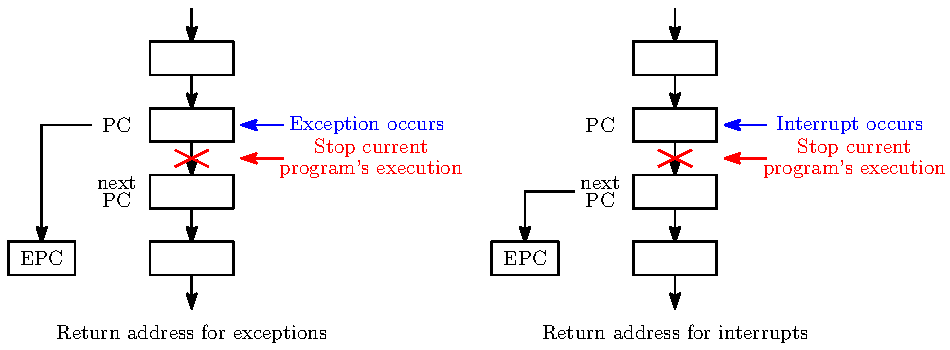
\includegraphics[width=\textwidth]{exceptions_EPC}
\caption{Return address in exceptions and interruptions.}
\label{Figure:exception_EPC}
\end{figure}
\end{frame}

% ========================================
% 
% ========================================
\begin{frame}{Exceptions \& Interrupts}{}
\begin{itemize}
\item \ac{MIPS} provides the special instruction \code{eret} for returning from exception handler.
\item This instruction writes into \ac{PC} the contents of \ac{EPC}.
\item If the offending instruction does not need to be executed again, the return address is incremented before being loaded into \ac{PC}.
\end{itemize}
\end{frame}

% ========================================
% 
% ========================================
\begin{frame}{Exceptions \& Interrupts}{}
\begin{itemize}
\item Interrupts may occur any time, even when the handler is executing an interrupt subroutine.
\item These further interrupt request may be enabled or disabled with a special control register.
\end{itemize}
\begin{figure}
\centering
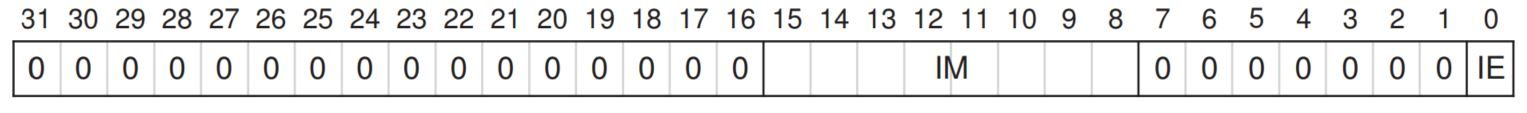
\includegraphics[width=\textwidth]{interrupt_masking}
\caption{Interrupt masking in Status register.}
\label{Figure:interrupt_masking}
\end{figure}
\begin{itemize}
\item The $i^{\mathrm{th}}$ bit in \code{IM} field represents the  $i^{\mathrm{th}}$ interruption request.
\item Bit \code{IE} is the global interrupt enable.
\item When an interrupt is attended, \ac{uP} may or may not disable (mask) all other \code{IM} bits, based on whether the \ac{uP} supports nested interrupts.
\end{itemize}
\end{frame}
% ========================================
% 
% ========================================
\begin{frame}{Exceptions \& Interrupts}{}
\begin{itemize}
\item If nested interrupts are supported, some states, including return addresses must be saved to the stack memory.
\item Moreover, some interrupts may have priority over others. For example, timers have priority over keyboard inputs.
\end{itemize}
\begin{figure}
\centering
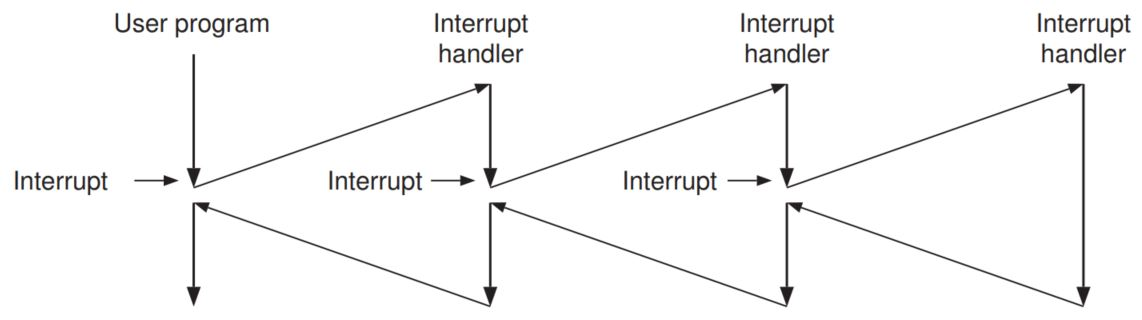
\includegraphics[width=\textwidth]{interrupt_nesting}
\caption{Interrupt nesting.}
\label{Figure:interrupt_nesting}
\end{figure}
\end{frame}

